\documentclass{article}

% Language setting
% Replace `english' with e.g. `spanish' to change the document language
\usepackage[english]{babel}

% Set page size and margins
% Replace `letterpaper' with `a4paper' for UK/EU standard size
\usepackage[letterpaper,top=2cm,bottom=2cm,left=3cm,right=3cm,marginparwidth=1.75cm]{geometry}

% Useful packages
\usepackage{amsmath}
\usepackage{graphicx}
\usepackage{ctex}
\usepackage[colorlinks=true, allcolors=blue]{hyperref}
\usepackage{listings}
\lstset{language=Matlab}
\begin{document}


\begin{figure}
	\centering
	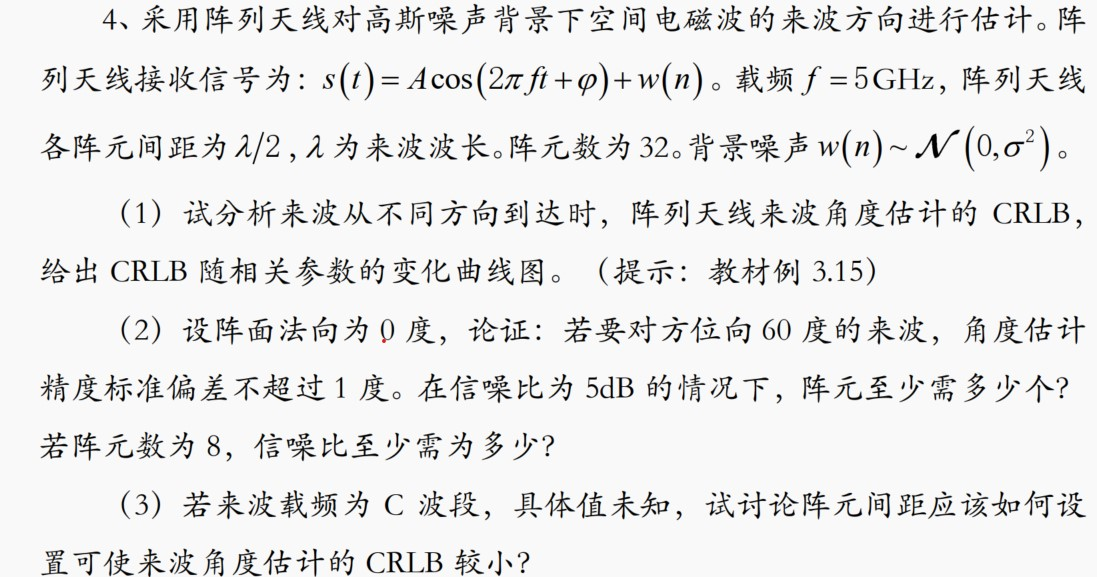
\includegraphics[width=1\linewidth]{4.jpg}
\end{figure}
解:
(1)由例题3.15可知,来波估计$\beta$的方差$var(\beta)$
\begin{equation}
	var(\beta) \geq \frac{12}{(2\pi)^{2}M\eta\frac{M+1}{M-1}(\frac{L}{\lambda})^{2}sin(\beta)^{2}}
	\tag{4.1}
\end{equation}
或
\begin{equation}
	var(\beta) \geq \frac{12}{(2\pi)^{2}M\eta\frac{M+1}{M-1}}\frac{c^2}{F_0^2d^2sin(\beta)^2} \tag{4.2}
\end{equation}
其中$$\eta=\frac{A^{2}}{2\sigma^{2}}$$

由式4.1可知$var(\beta)$和$\beta$、阵元数M、信噪比$\eta$以及阵元宽度和波长之比有关,用matlab绘制他们之间曲线

\begin{itemize}
	\item 设置入射角$0<\beta<\pi$,CRLB和入射角之间的关系如下图1

\end{itemize}

\begin{figure}
	\centering
	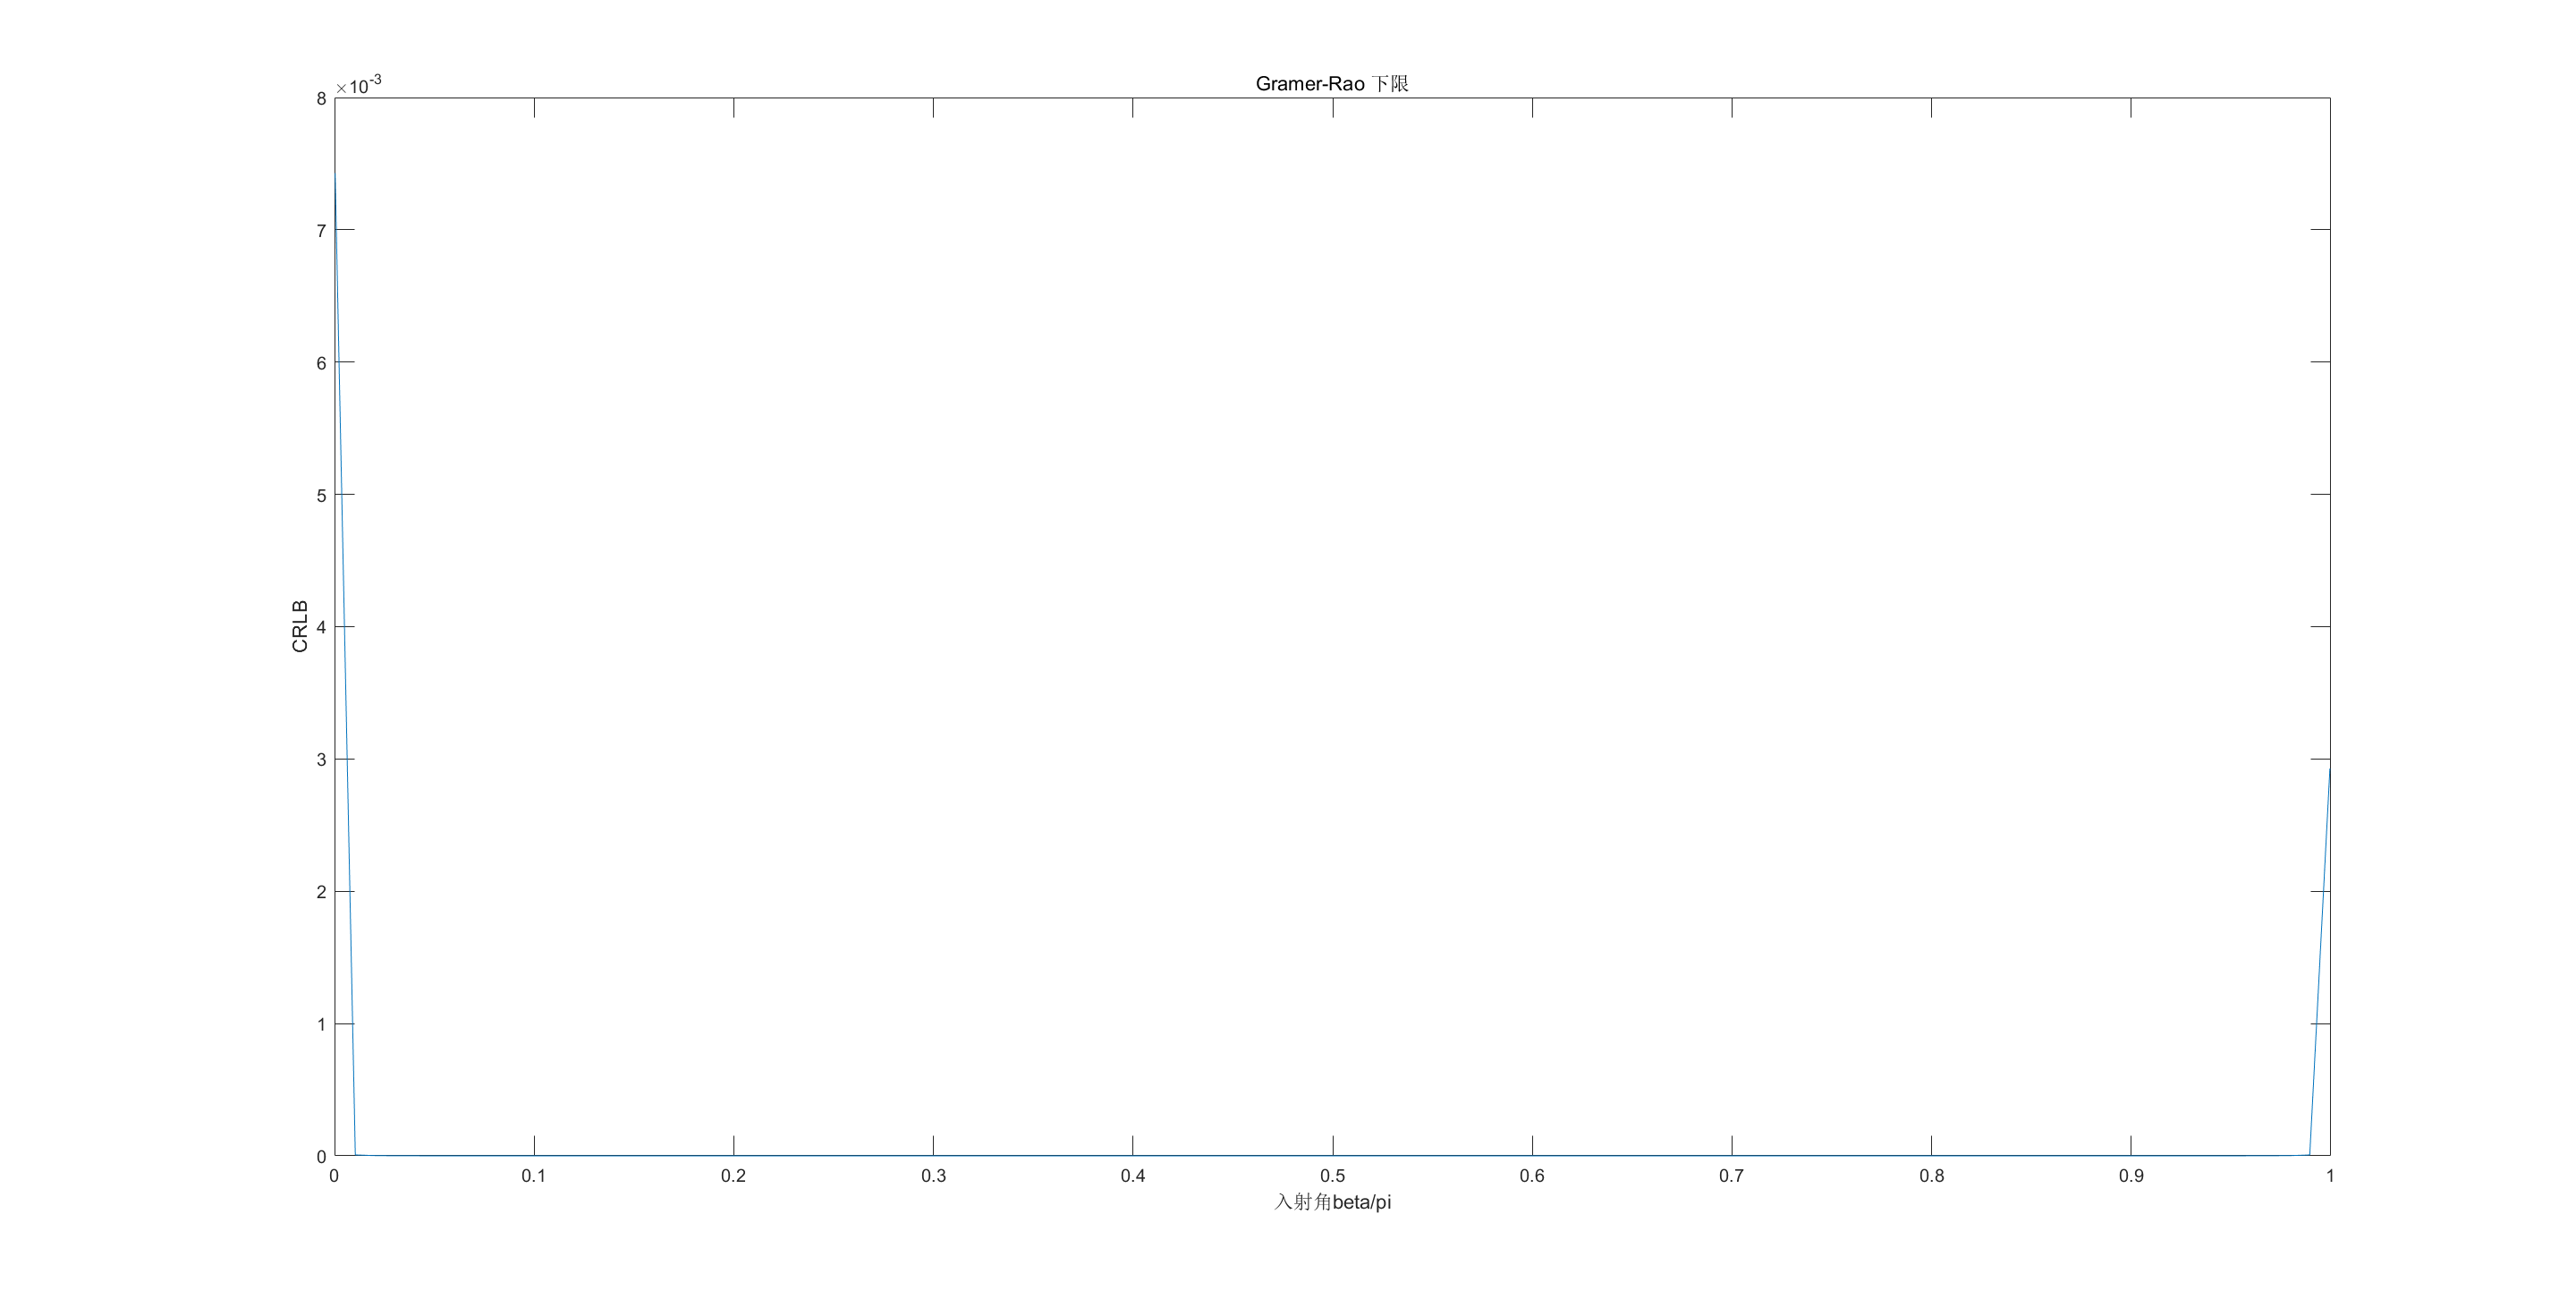
\includegraphics[width=0.75\linewidth]{CRLB 入射角.png}
	\caption{CRLB和入射角之间的关系}

\end{figure}
由图2可知,当$\beta$大于某项值时,CRLB $\to 0$,图像关于$\frac{\pi}{2}$对称,当$\beta \to 0 或 \pi 时$,CRLB $\to \infty$这是因为靠近入射面时,测量误差很大。
\begin{itemize}
	\item 当入射角固定为30°时,设置信噪比$\eta$在[0.001  100]之间变化
\end{itemize}

\begin{figure}
	\centering
	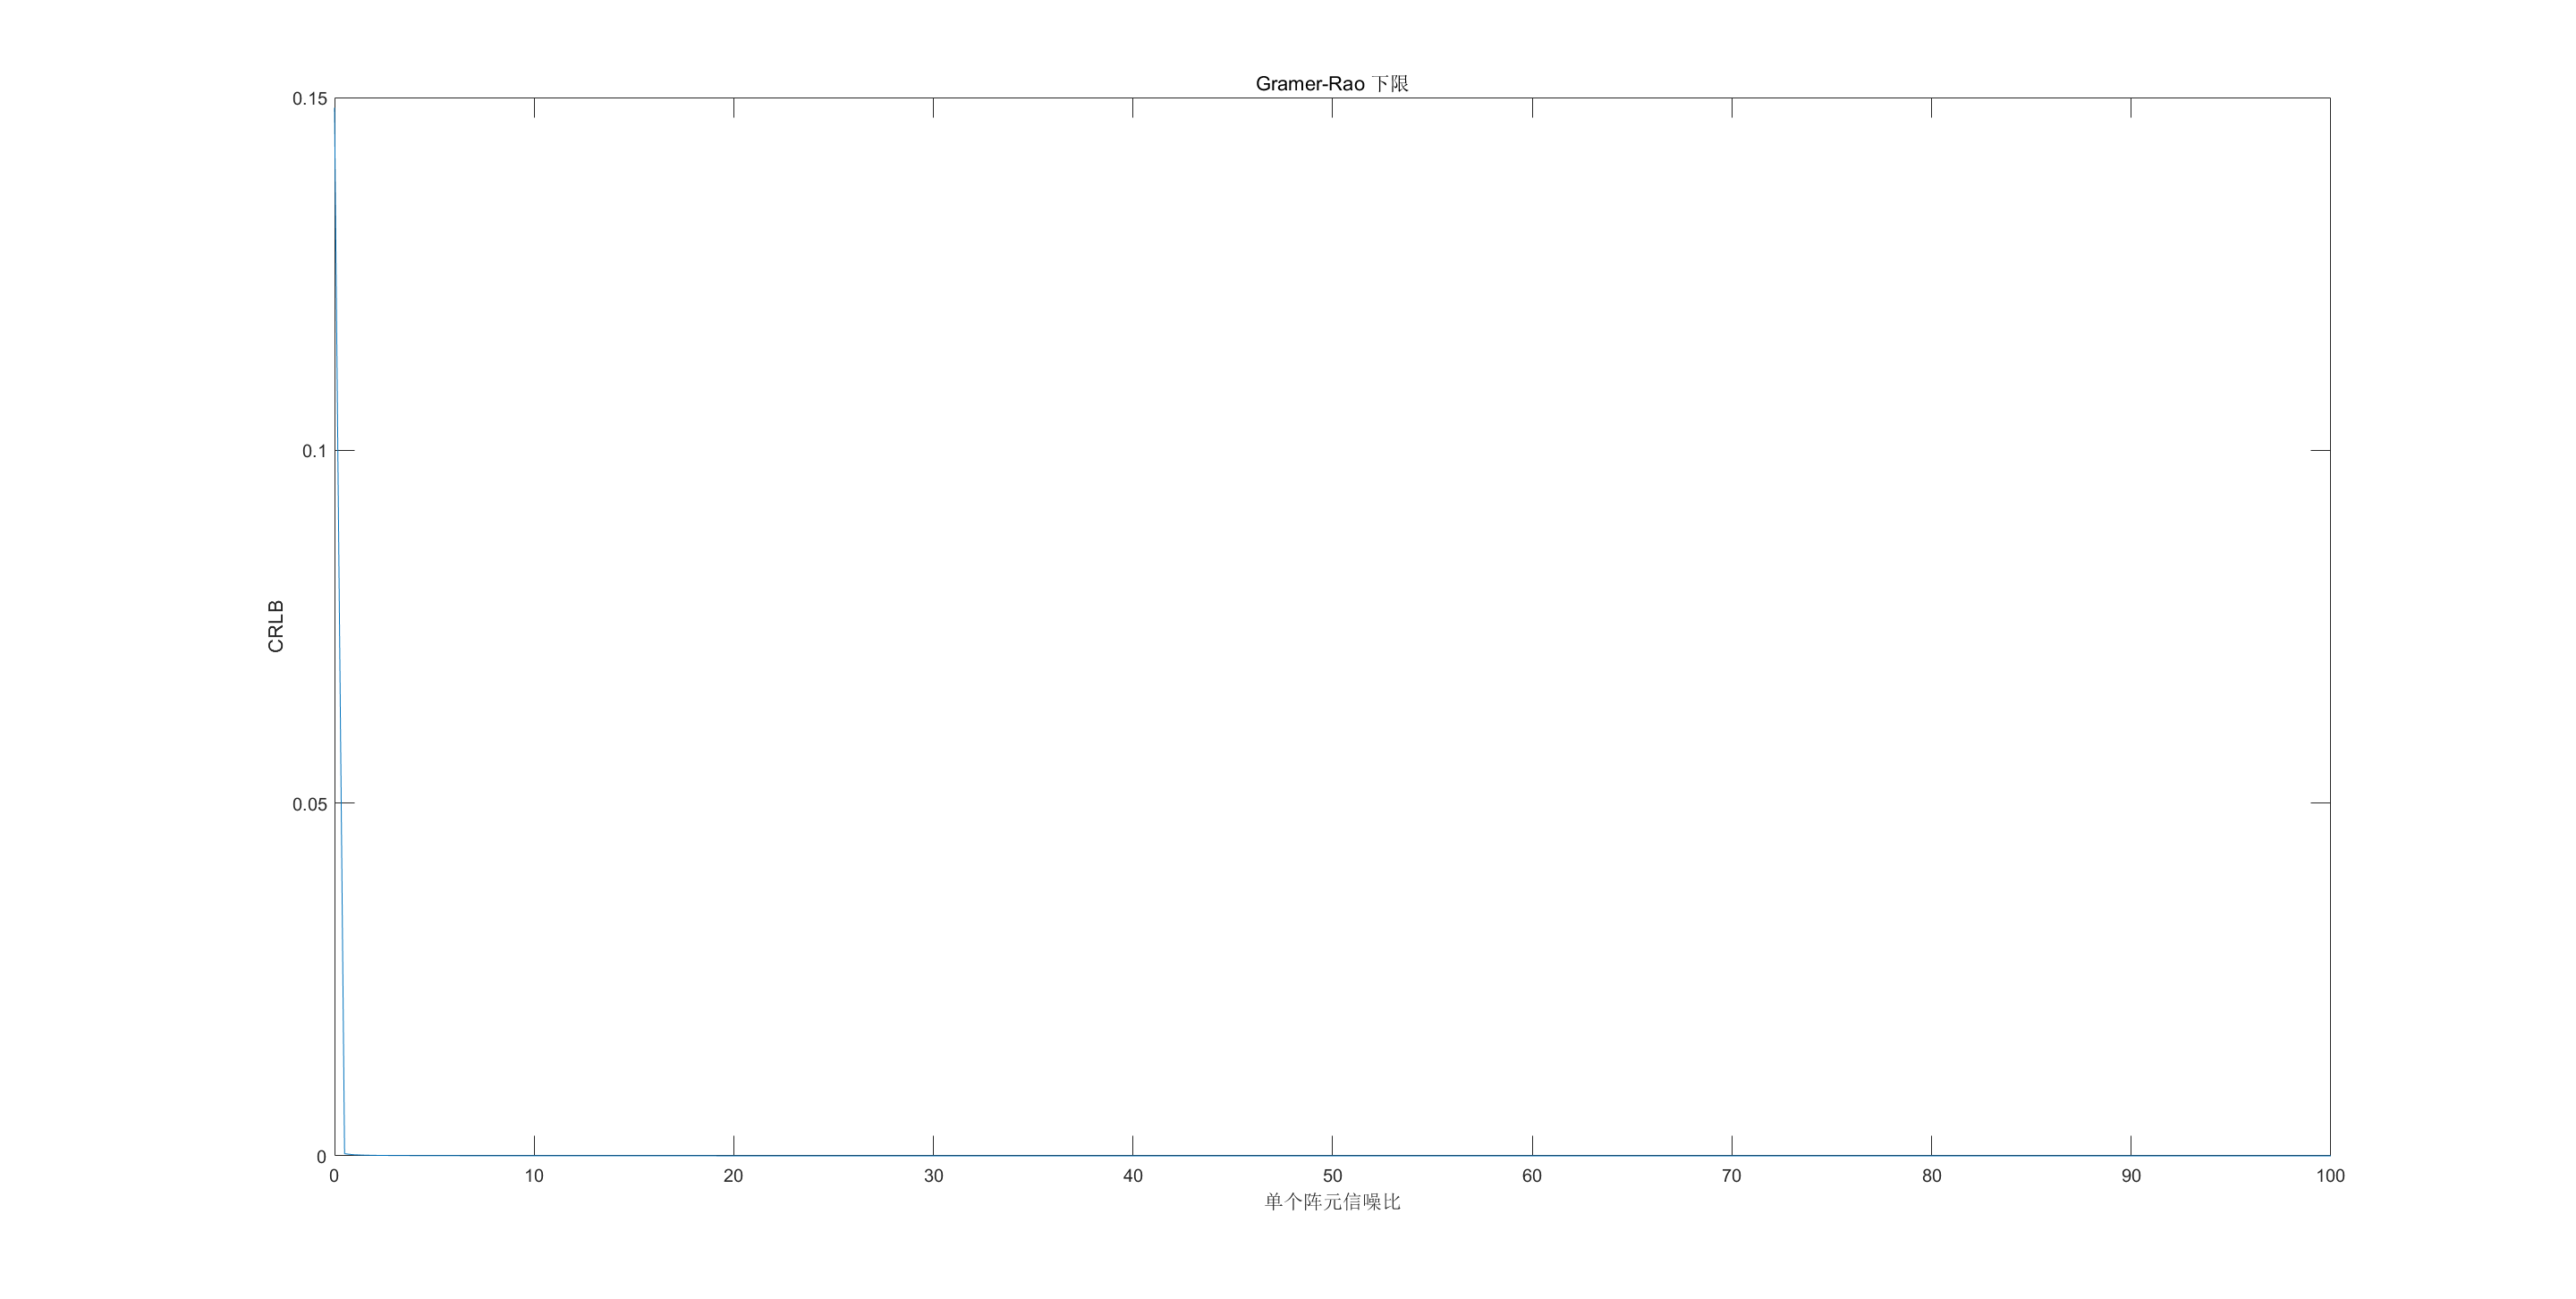
\includegraphics[width=0.75\linewidth]{CRLB 信噪比eta.png}
	\caption{CRLB信噪比$\eta$关系}

\end{figure}
由图像可知,当信噪比$\eta \to \infty$ 时,$CRLB \to 0$,测量误差变小
\begin{itemize}
	\item 设置M从2至50之间变化,入射角固定为30,信噪比$\eta =5dB$时,RLB和入射角之间的关系如下
\end{itemize}
\begin{figure}
	\centering
	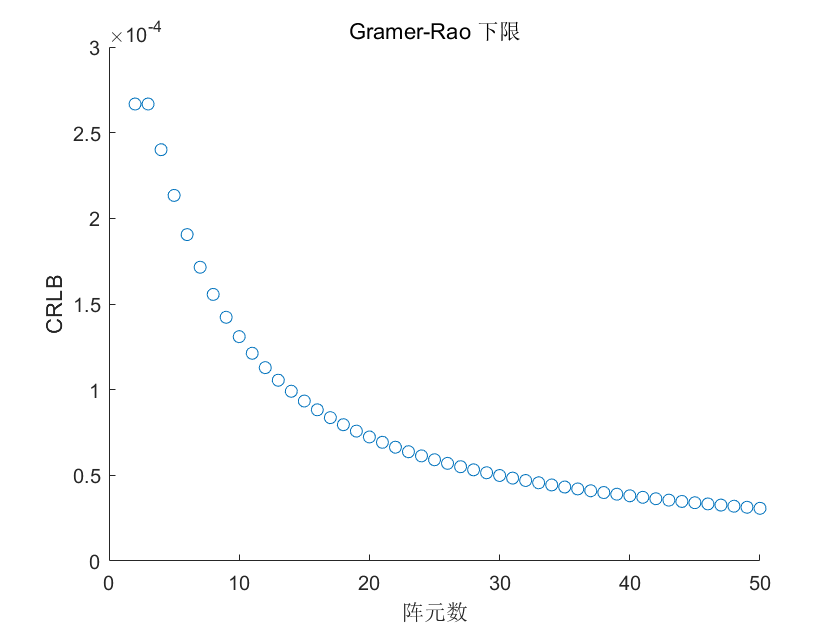
\includegraphics[width=0.75\linewidth]{CRLB 阵元数.png}
	\caption{CRLB和阵元M之间关系}


\end{figure}
由图3可知,当阵元数$M$增加 时,$CRLB$减小,且在阵元为2时,即$CRLB$小于0
\begin{itemize}
	\item 设置阵元为8,入射角固定为30度时,CRLB和阵元长度与波长之比之间的关系如下
\end{itemize}
\begin{figure}
	\centering
	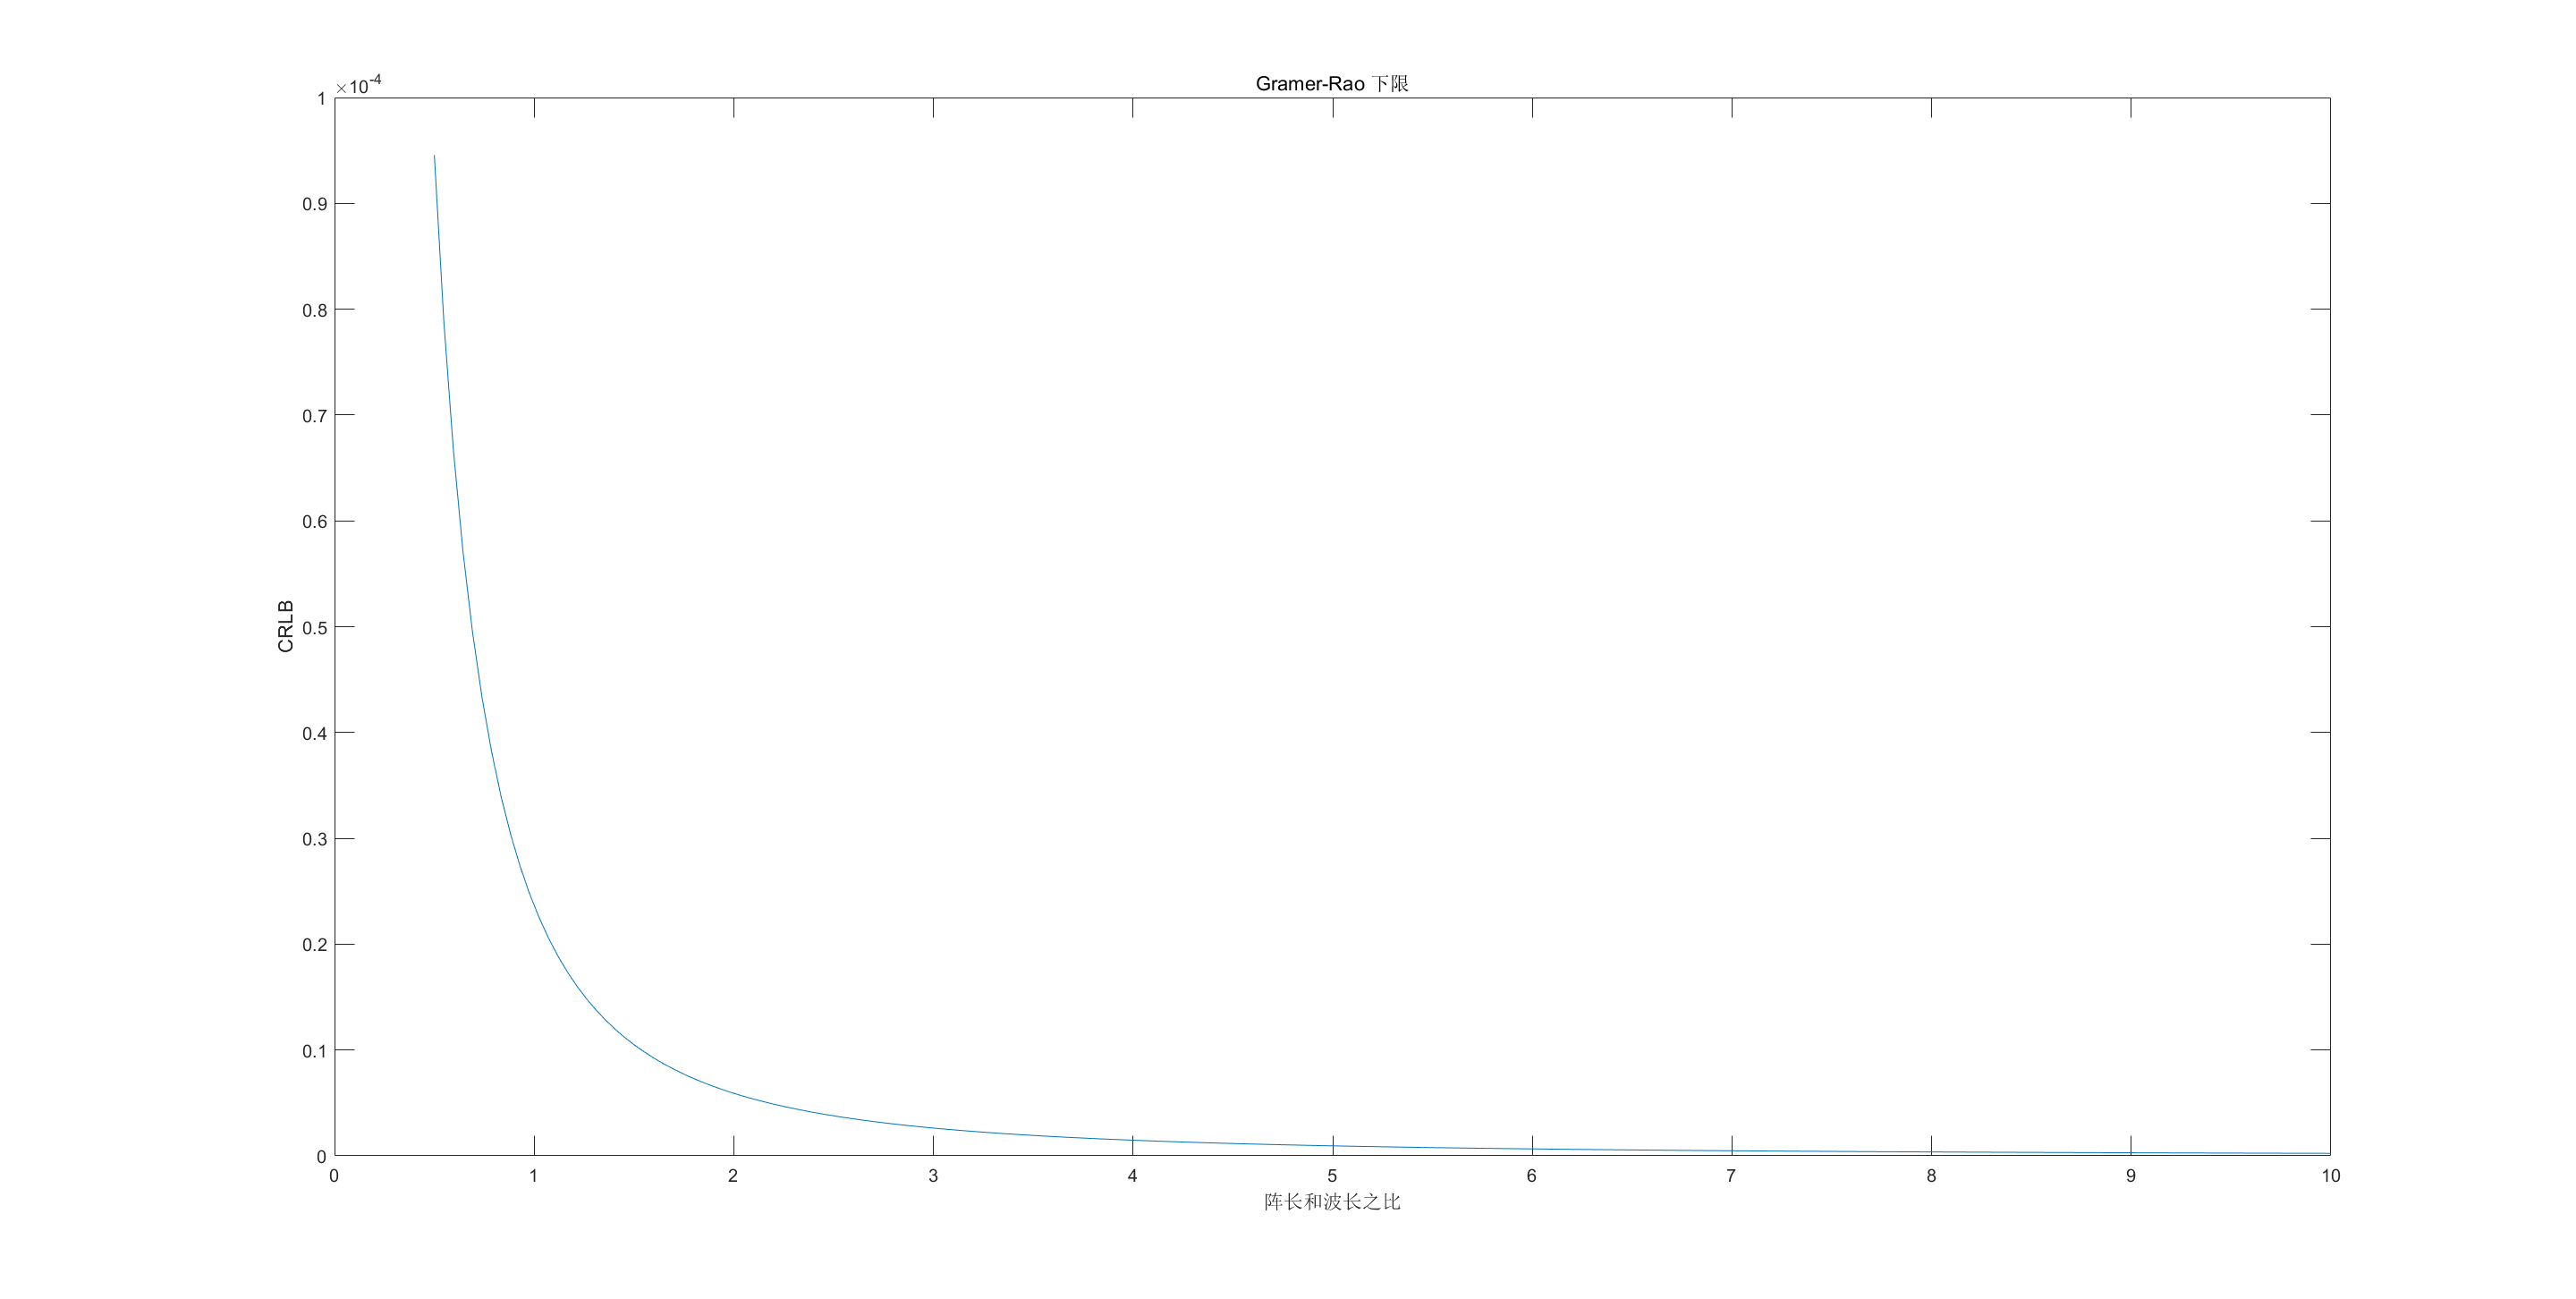
\includegraphics[width=0.75\linewidth]{CRLB 波长比.png}
	\caption{CRLB和阵元长度和波长之比关系}


\end{figure}
有图4可知,随着阵元数增加,阵元长和$\lambda$之比增加,$CRLB减少$

(2)相对阵面入射角度 $\beta=\frac{\pi}{6}$,
信噪比 $10log(\eta)=5dB$
则$\eta$ =3.1623
$\beta$估计偏差小于1°,即$var(\beta)\leq$1;
有上面讨论和M绘制的关系图发现,M=2即可满足条件。
当$M$=8时,若$var(\beta)$小于1,
则求得$eta$=0.804

(3)若来波为C波段,则中心频率$f_0$在4-8GHz,若使$var(\beta)$,由式4.2可知$F_0$
越大,$d$越大,或$\frac{\lambda}{d}$越小($\lambda$越小,$d$越大),则$var(\beta)$越小,即
$$0<\frac{F_0d}{c}cos\beta=\frac{d}{\lambda}cos\beta<\frac{1}{2}$$
则$d$最大取$\frac{\lambda}{2}$,$\lambda$对应为8Ghz时最小,此时$\lambda$=0.0375m

附:matlab代码

\begin{lstlisting}
close all
%按照题目所给数据设置仿真参数
c=3e8;
f0 = 5e9;%中心频率5G
M = 32;%阵元数32
A=1;
sigma2 = 0.01;
eta= 0.5*A^2/sigma2^2; %信噪比
beta=linspace(0.001,3.14,100);%入射角
lambda = c/f0;%入射信号波长
d = 0.5*lambda; %孔径间距
L_lambda = (M-1)*d/lambda;%L/lambda 之比,L阵的长度(M-1)d

%CRLB of beta 入射角的CRLB 
y1=4*pi^2*M*eta*(M+1)/(M-1)*L_lambda^2.*sin(beta).^2;
y=12./y1;
%绘制CRLB和入射角之间的图形
figure(1)
plot(beta/pi,y)
xlabel('入射角beta/pi');
ylabel('CRLB');
title('Gramer-Rao 下限')

%%当入射角为60度(相对阵面方向为30度)时CRLB和信噪比eta 的关系
beta=pi/6;%入射角为30°
eta=linspace(0.001,100,200);
y1=4*pi^2*M*eta*(M+1)/(M-1)*L_lambda^2.*sin(beta).^2;
y=12./y1;
figure(2)
plot(eta,y);
xlabel('单个阵元信噪比');
ylabel('CRLB');
title('Gramer-Rao 下限')

%%当入射角为60度(相对阵面方向为30度)时CRLB和阵元数量M 的关系
beta=pi/6;%相对阵面方向为30度
M = 2:1:50;
eta=3.1623%信噪比即为5dB;
y1=4*pi^2.*M*eta.*(M+1)./(M-1)*L_lambda^2.*sin(beta).^2;
y=12./y1;
figure(3)
scatter(M,y);
xlabel('阵元数');
ylabel('CRLB');
title('Gramer-Rao 下限')

%%当入射角为60度(相对阵面方向为30度)时CRLB和阵的长度和波长之比L_lambda 的关系
beta=pi/6;%入射角设定为30°
L_lambda=linspace(0.5,15,200);
eta= 0.5*A^2/sigma2^2; %信噪比
M=8;
y1=4*pi^2*M*eta*(M+1)/(M-1).*L_lambda.^2.*sin(beta).^2;
y3=12./y1;
figure(4)
plot(L_lambda,y3);
xlabel('阵长和波长之比');
ylabel('CRLB');
title('Gramer-Rao 下限')
\end{lstlisting}

\end{document}


